\setlength{\footskip}{8mm}

\chapter{Methodology}
\label{ch:methodology}

\section{Data Set}

\subsection{Description}
The primary dataset used in this project is a merged hydro-meteorological time series created by integrating three distinct sources:

\begin{itemize}
    \item \textbf{1. Water Level Data (Station CPY015)}

    This dataset\cite{hiiwaterlevel} originates from the \textbf{Thai Water Reporting System (Hydro-Informatics Institute)} and contains hourly water level measurements in meters above Mean Sea Level (m.MSL). Station CPY015 is located at latitude 13.7361 and longitude 100.5464, with reference values including Ground Level (1.951 m.MSL), Bank Level (2.161 m.MSL), and Bed Level (-15.70 m.MSL).

    \item \textbf{2. Meteorological Data (Open-Meteo)}

    To enrich the hydrological records, historical weather data were retrieved through the Open-Meteo archive API\cite{openmeteo} and provides hourly observations for the following meteorological variables:
    \begin{itemize}
        \item \texttt{temperature\_2m}
        \item \texttt{rain}
        \item \texttt{showers}
        \item \texttt{relative\_humidity\_2m}
        \item \texttt{pressure\_msl}
        \item \texttt{wind\_speed\_10m}
        \item \texttt{et0\_fao\_evapotranspiration}
    \end{itemize}

    \item \textbf{3. River Discharge Data (Open-Meteo Flood API)}

    Upstream flow conditions were captured using the Open-Meteo Flood API, which provides modeled river discharge estimates in $m^3/s$. Discharge values were sampled near the station location and merged with water level and weather data through time-based interpolation to align with the prediction timeline.
\end{itemize}

\subsection{Key Feature Groups}
\begin{itemize}
    \item \textbf{Hydrological Features:}
    Includes \texttt{river\_discharge}, \texttt{water\_level}, and derived lag features at 1, 2, 3, 6, 12, and 24 hours.

    \item \textbf{Rolling Statistics:}
    To capture recent trends and variability, rolling \texttt{mean}, \texttt{std}, \texttt{min}, and \texttt{max} statistics were calculated over windows of 6, 12, and 24 hours.

    \item \textbf{Difference Features:}
    Rate of change features were generated by calculating the difference between the current water level and values from 1 hour and 24 hours prior.

    \item \textbf{Temporal Features:}
    To capture cyclical patterns (daily tides and seasonal monsoons), temporal values (hour of day, month) were encoded using sine and cosine transformations.
\end{itemize}

\textbf{Target Labels:}
\begin{itemize}
    \item \textbf{Primary Output:} \texttt{water\_level} (continuous value in m.MSL) predicted 24 hours into the future.
    \item \textbf{Secondary Output:} Risk classification (Low, Medium, High, Critical) as detailed in Section \ref{sec:risk_standards}.
\end{itemize}

\subsection{Risk Classification Standards}
\label{sec:risk_standards}
To provide actionable early warnings, predicted water levels are mapped to risk categories based on the station's hydraulic capacity. This classification logic is adapted from the \textbf{ThaiWater} reporting standards (Hydro-Informatics Institute)\cite{thaiwater_wl}.

For Station CPY015 (Krungthep Bridge), the risk level is determined by the percentage of effective bank capacity utilized:
\begin{equation}
    \text{Capacity \%} = \frac{\text{Water Level} - \text{Bed Level}}{\text{Bank Level} - \text{Bed Level}} \times 100
\end{equation}
where:
\begin{itemize}
    \item \textbf{Bank Level:} 2.161 m.MSL (Critical overflow point)
    \item \textbf{Bed Level:} -15.70 m.MSL (River bottom)
\end{itemize}

The resulting percentages are classified as follows:
\begin{itemize}
    \item \textbf{Critical ($\ge 90\%$):} Imminent flood danger. Water level is near or above bank capacity.
    \item \textbf{High Risk ($70-90\%$):} Warning level. Significant rise requiring monitoring.
    \item \textbf{Medium Risk ($30-70\%$):} Normal to elevated levels.
    \item \textbf{Low Risk ($< 30\%$):} Safe operating levels.
\end{itemize}

\section{Data Acquisition}

The dataset for this study was constructed by combining in-situ river water level measurements with meteorological and discharge estimates into a unified hourly time series. Water level records were collected from Station CPY015 through the Hydro-Informatics Institute platform, while historical weather data and discharge estimates were retrieved using Open-Meteo APIs. All sources were aligned to a consistent hourly frequency, spanning January 2019 to May 2025, resulting in over 56,000 hourly observations.

\section{Exploratory Data Analysis (EDA)}

The final merged dataset consists of 56,232 hourly records spanning over six years. Comprehensive analysis reveals critical hydrological patterns that inform our modeling strategy.

\subsection{Temporal Patterns and Seasonality}
The water level time series (Figure \ref{fig:water_level_ts}) exhibits distinct seasonal cyclicity driven by Thailand's monsoon seasons. Annual peaks consistently occur between September and November, corresponding to the late rainy season and high river discharge periods. Conversely, dry seasons (December to April) show stable, lower water levels. These strong seasonal components confirm the necessity of including time-based features (month, day of year) and long-term lag features to capture annual periodicity.

\begin{figure}[htbp]
    \centering
    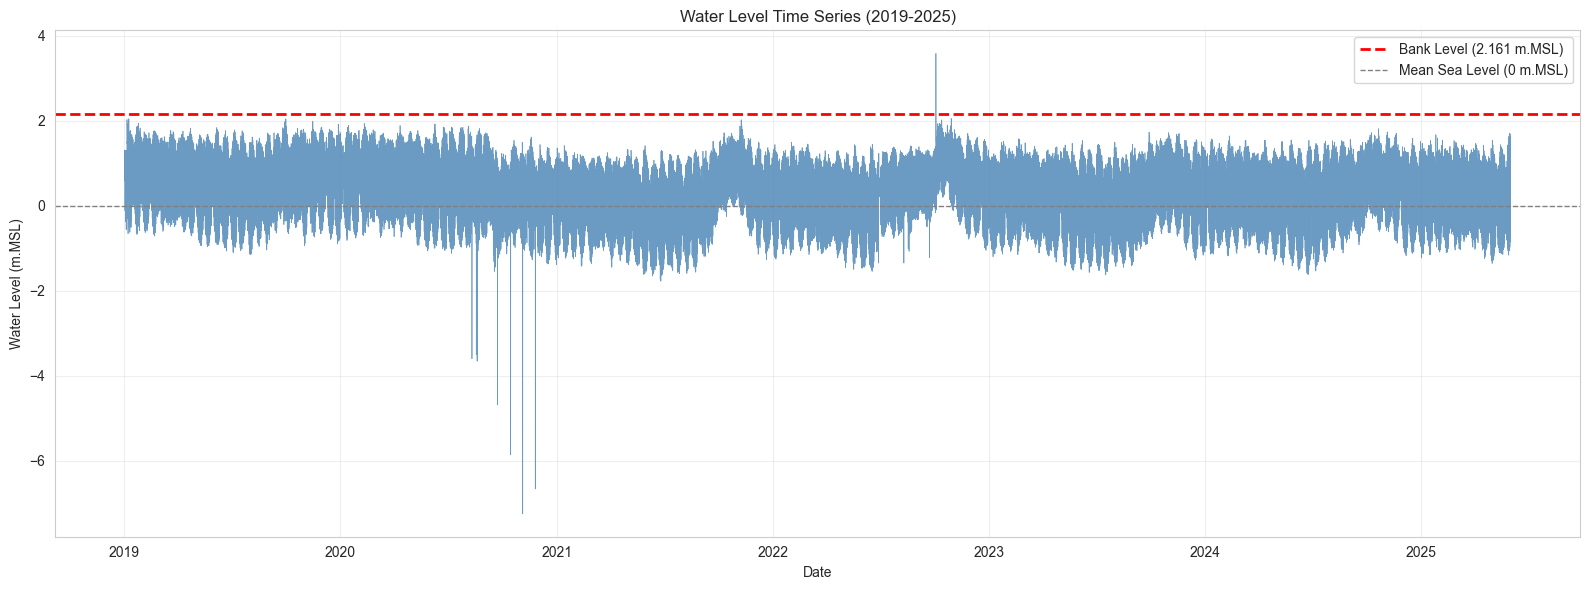
\includegraphics[width=0.9\textwidth]{figures/water_level_2019_2025.png}
    \caption{Water Level Time Series (2019-2025).}
    \label{fig:water_level_ts}
\end{figure}

\subsection{Feature Relationships}
Correlation analysis (Figure \ref{fig:correlation_matrix}) quantifies the drivers of water level changes. We observed a strong positive correlation ($r=0.85$) between water level and \texttt{river\_discharge}, confirming that upstream flow is the primary physical driver. Rainfall variables show moderate positive correlation ($r \approx 0.45$), acting as secondary contributors. The Pair Plot (Figure \ref{fig:pair_plot}) further reveals that these relationships are often non-linear, particularly at extreme values, which justifies the use of deep learning models like LSTM over simple linear regression.

\begin{figure}[htbp]
    \centering
    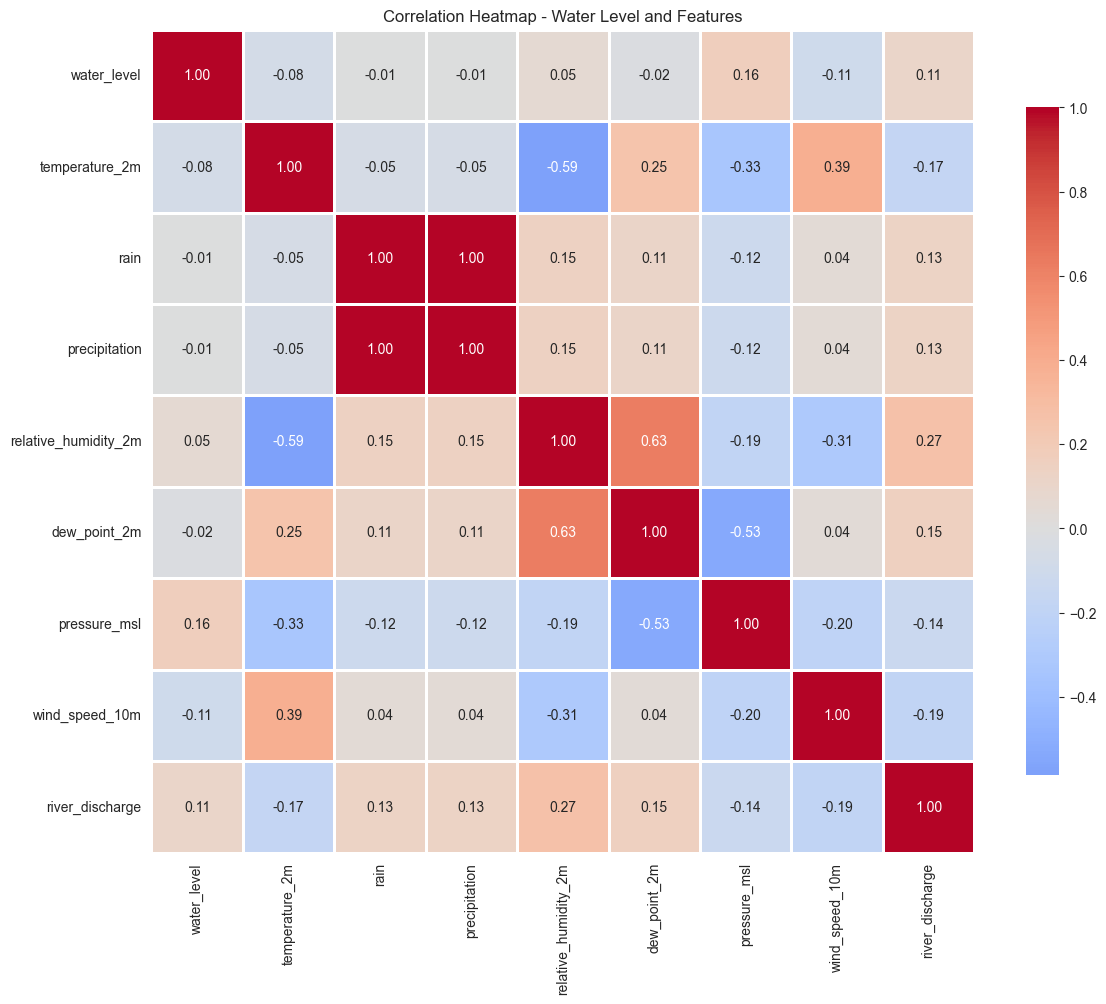
\includegraphics[width=0.8\textwidth]{figures/correlation_matrix.png}
    \caption{Correlation Matrix of hydrological and meteorological variables.}
    \label{fig:correlation_matrix}
\end{figure}

\begin{figure}[htbp]
    \centering
    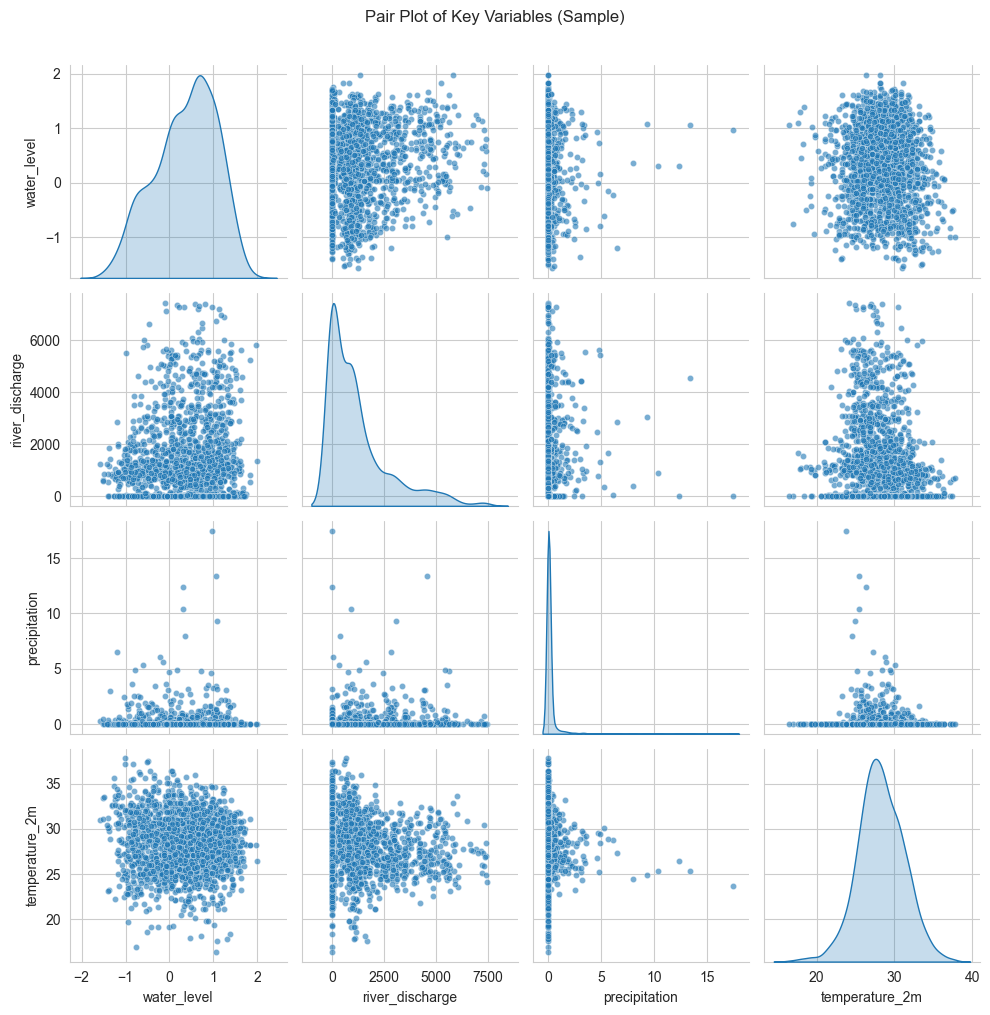
\includegraphics[width=0.9\textwidth]{figures/pair_plot_key_variable.png}
    \caption{Pair Plot illustrating non-linear feature interactions.}
    \label{fig:pair_plot}
\end{figure}

\subsection{Distribution and Risk Profile}
The distribution of water levels is slightly negatively skewed and not normally distributed (Shapiro-Wilk test $p < 0.05$), with a total range of 4.42 meters (-2.48 to 1.94 m.MSL). When mapped to risk zones (Figure \ref{fig:risk_dist}), the data shows a significant class imbalance: the vast majority of hours fall into "Low" or "Medium" risk categories, while "High" and "Critical" events are rare tail events. This imbalance poses a challenge for predictive modeling, requiring robust training strategies to ensure the model learns to predict these rare but critical flood events accurately.

\begin{figure}[htbp]
    \centering
    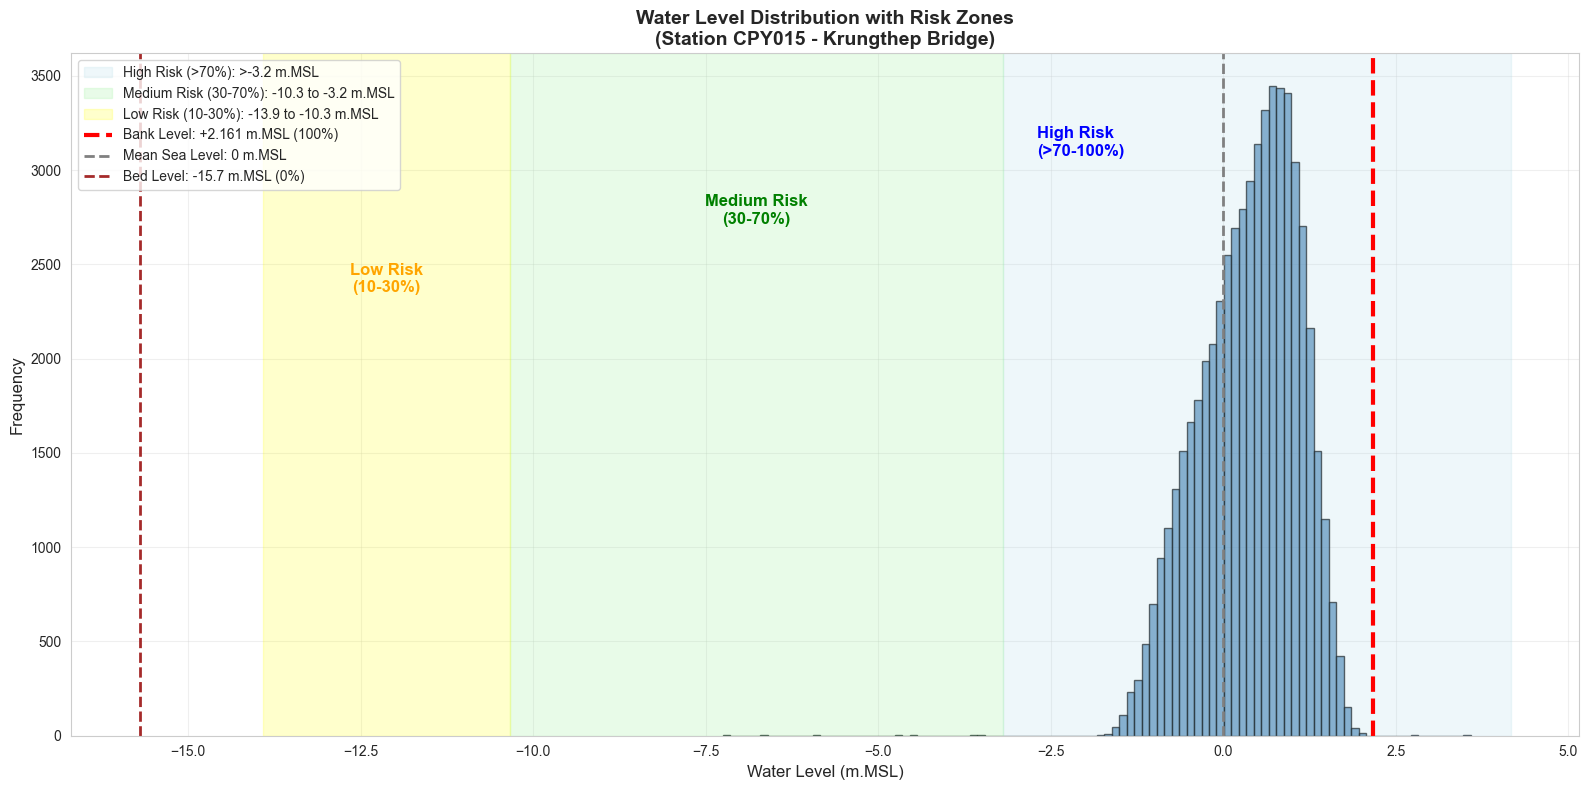
\includegraphics[width=0.8\textwidth]{figures/water_level_distribution_with_risk_zone.png}
    \caption{Water Level Distribution stratified by Risk Zones.}
    \label{fig:risk_dist}
\end{figure}

Overall data quality is high, with less than 0.5\% missing values across all features.

\subsection{Rationale for Meteorological Integration}
A critical design decision in this study was the integration of meteorological data, despite the strong autoregressive nature of water levels. While historical water level data effectively captures seasonal trends (monsoon cycles) and daily tidal patterns, it lacks the ability to predict sudden deviations caused by external forcing. Meteorological variables serve as \textbf{leading indicators}:
\begin{itemize}
    \item \textbf{Rainfall (Precipitation):} Acts as the primary driver of surface runoff. Heavy rainfall signals a future rise in water levels with a lag time of 6-24 hours, allowing the model to anticipate floods before the water level physically rises.
    \item \textbf{Atmospheric Pressure:} Low-pressure systems are precursors to storm surges and can alter tidal behaviors.
    \item \textbf{Humidity \& Temperature:} These variables indicate evaporation rates and soil saturation levels. High humidity and low temperature suggest reduced evaporation, leading to faster runoff and higher water retention.
\end{itemize}
By incorporating these "causal" features, the model transitions from simple trend extrapolation to physically-informed forecasting.

\section{Model Implementation and Training}

\subsection{Model Selection}
To establish a robust benchmark and justify the use of deep learning, we implemented a diverse set of models ranging from simple heuristics to advanced ensemble methods:

\subsubsection{Baseline Models}
\begin{itemize}
    \item \textbf{Persistence Model:} Assumes the future state will be identical to the current state. This serves as the lower bound for performance.
    \begin{equation}
        \hat{y}_{t+24} = y_t
    \end{equation}
    
    \item \textbf{Seasonal Naive:} Assumes the future state will repeat the value from exactly 24 hours ago, capturing daily tidal cycles.
    \begin{equation}
        \hat{y}_{t+24} = y_{t-24}
    \end{equation}
    
    \item \textbf{Rolling Mean:} Predicts the average of the last 24 hours.
    \begin{equation}
        \hat{y}_{t+24} = \frac{1}{24}\sum_{i=0}^{23} y_{t-i}
    \end{equation}
\end{itemize}

\subsubsection{Machine Learning Models}
\begin{itemize}
    \item \textbf{Linear \& Ridge Regression:} Used to model linear relationships between features and the target. Ridge regression adds L2 regularization to handle multicollinearity among correlated weather features.
    \item \textbf{XGBoost \& LightGBM:} Gradient boosting decision tree algorithms that excel at capturing non-linear interactions and handling tabular data. They provide feature importance scores and are robust to outliers.
\end{itemize}

\subsection{LSTM Architecture}
The core of our predictive system is a Long Short-Term Memory (LSTM) network, designed to capture temporal dependencies in the time-series data. The LSTM unit addresses the vanishing gradient problem using a gating mechanism defined by the following equations:

\begin{equation}
    \begin{aligned}
        f_t &= \sigma(W_f \cdot [h_{t-1}, x_t] + b_f) \\
        i_t &= \sigma(W_i \cdot [h_{t-1}, x_t] + b_i) \\
        \tilde{C}_t &= \tanh(W_C \cdot [h_{t-1}, x_t] + b_C) \\
        C_t &= f_t \cdot C_{t-1} + i_t \cdot \tilde{C}_t \\
        o_t &= \sigma(W_o \cdot [h_{t-1}, x_t] + b_o) \\
        h_t &= o_t \cdot \tanh(C_t)
    \end{aligned}
\end{equation}

where $x_t$ is the input vector, $h_t$ is the hidden state, $C_t$ is the cell state, and $\sigma$ is the sigmoid activation function.

The architecture, implemented in PyTorch, consists of the following components:
\begin{itemize}
    \item \textbf{Input Layer:} Accepts a sequence of feature vectors with shape $(Batch, Sequence\_Length, Input\_Features)$.
    \item \textbf{LSTM Layer:} A single LSTM layer with \texttt{hidden\_size=128} and \texttt{batch\_first=True}.
    \item \textbf{Dropout Layer:} A dropout rate of $0.3$ is applied to prevent overfitting.
    \item \textbf{Fully Connected Layer:} Maps the final hidden state to the predicted water level.
\end{itemize}

\subsection{Evaluation Metrics}
To rigorously assess model performance, we employed the following metrics:

\begin{itemize}
    \item \textbf{Mean Absolute Error (MAE):} Measures the average magnitude of errors.
    \begin{equation}
        MAE = \frac{1}{n}\sum_{i=1}^{n}|y_i - \hat{y}_i|
    \end{equation}
    
    \item \textbf{Root Mean Squared Error (RMSE):} Penalizes larger errors more heavily.
    \begin{equation}
        RMSE = \sqrt{\frac{1}{n}\sum_{i=1}^{n}(y_i - \hat{y}_i)^2}
    \end{equation}
    
    \item \textbf{Coefficient of Determination ($R^2$):} Represents the proportion of variance explained by the model.
    \begin{equation}
        R^2 = 1 - \frac{\sum_{i=1}^{n}(y_i - \hat{y}_i)^2}{\sum_{i=1}^{n}(y_i - \bar{y})^2}
    \end{equation}
\end{itemize}

\subsection{Hyperparameters}
The model was trained with the following hyperparameters:
\begin{itemize}
    \item \textbf{Sequence Length:} 48 hours
    \item \textbf{Hidden Size:} 128 units
    \item \textbf{Number of Layers:} 1
    \item \textbf{Dropout:} 0.3
    \item \textbf{Batch Size:} 64
    \item \textbf{Learning Rate:} 0.001
    \item \textbf{Optimizer:} Adam
    \item \textbf{Loss Function:} Mean Squared Error (MSE)
    \item \textbf{Epochs:} 50 (with early stopping)
\end{itemize}

\subsection{Training Strategy}
To ensure robust performance and prevent data leakage, we employed a strict training pipeline:

\begin{enumerate}
    \item \textbf{Time Series Cross-Validation:} We used \texttt{TimeSeriesSplit} with 5 splits. This ensures that the model is always trained on past data and validated on future data, respecting the temporal order.
    \item \textbf{Fold-Safe Preprocessing:} Feature scaling (\texttt{StandardScaler}) was fitted \textit{only} on the training portion of each fold and then applied to the validation portion. This prevents information from the validation set (future) from leaking into the training process.
    \item \textbf{Early Stopping:} Training was monitored using the validation loss. If the validation loss did not improve for 10 consecutive epochs, training was halted to prevent overfitting.
    \item \textbf{Gradient Clipping:} Gradients were clipped to a maximum norm of 1.0 to prevent exploding gradients, a common issue in RNN training.
\end{enumerate}
8+ with the following key libraries:
\begin{itemize}
    \item \textbf{Data Processing:} Pandas, NumPy
    \item \textbf{Machine Learning:} Scikit-learn, XGBoost, LightGBM
    \item \textbf{Deep Learning:} PyTorch (for LSTM)
    \item \textbf{Visualization:} Matplotlib, Seaborn, Plotly
    \item \textbf{Web Application:} Streamlit
\end{itemize}

The training pipeline involved a 5-fold TimeSeriesSplit Cross-Validation to ensure temporal integrity. All models were trained on an 80/20 train-test split, with the training set covering January 2019 to February 2024, and the test set covering February 2024 to May 2025.
